At this point, I will have identified a set of suitable quality indicators for heart failure at the MUHC and have two \gls{EAF} systems with validated usability and usefulness: a gamified, and a traditional system. I will use these systems to estimate how a behavioural intervention focused on intrinsic motivators (i.e., using the principles of gamification), affects adoption, engagement, and effectiveness of an e-A\&F intervention.

The proposed research design is a single center, parallel-arm, actively controlled randomized control trial (\gls{RCT}) of physicians treating heart failure patients at the \gls{MUHC}. Random assignment will use a 1:1 ratio. Both systems will present feedback based on the quality measures in objective 1. The trial is planned to last 14 months in total. The RCT design was chosen as opposed to an impact evaluation to increase the usefulness of the results it generates by aligning more closely with prior evidence in the field. The intervention will be delivered through a personalized, confidential web-based portal, accessible by navigating to a specific URL on a ward computer or personal device. In this objective, my hypothesis is that there is a difference in adoption of the \gls{EAF} system between the traditionally designed and gamified arms. Similarly, I hypothesize a difference in engagement between the arms. The null hypotheses being that there is no difference in adoption or engagement. I consider effectiveness a secondary objective in this trial as the true effect of the systems might be affected by their adaptation, the length of the trial, or what quality measure our data support.

\begin{figure}[h]
    \centering
    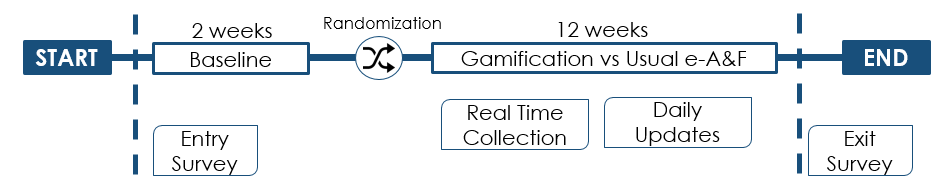
\includegraphics[width=\textwidth]{img/rct_flow.png}
    \caption{Diagram of the RCT process}
    \label{fig:rct_flow}
\end{figure}

\section{Timing, Participants, and Consent}
To participate in this trial, users must be physicians working at the MUHC, have control over the treatment of patients with heart failure, and have worked in the emergency department (ED) or in the intensive care unit (ICU) for at least 10 weeks\footnote{Baseline assessment + 2 months}. This population will include attending physicians, medical residents, and fellows. Participants will be followed for a maximum of 12 weeks after the mandatory 2 weeks baseline assessment. The choice of 12 weeks was made by balancing feasibility with the need for participants and for enough follow-up to measure retention. No recruitment will be attempted in the last 2 months of the trial. Recruitment will be made by informing the different departments, with recruitment material, and with a local advocate. An email reminder will be sent every 90 days to recommend users to login. Ongoing monitoring will be performed for any signs of harm to patients.

% Consent Process
Since only secondary patient data is used, and since it is used as part of the care process, a waiver of patient consent will be requested from the director of professional services. Informed consent will be required from each participating physician and they can stop using either intervention at any time. Participants will not be allowed to switch between arms. If participants inform us of their desire to stop using the interventions, an exit survey will be sent to them.

\section{Data Collection}
No \textit{patient} data will be captured specifically for this project. Patient data are used only to create provider-level feedback. Providers will be able to see nominative data for themselves and their own patients. Both systems will automate indicator processing from patient data as described in the ``data source'' section. Simple randomization will be performed with a 1:1 ratio after a user fills in the entry questionnaire. Both systems will perform real-time data collection as participants use them. Data will be recorded in a secured database, assigned to the anonymous ID of the participant. Participant quality measures will be confidential and will not be shared. All analysis will be performed on participant's anonymous IDs. Participant data will be stored for a duration of 7 years, and any identifier will be removed as soon as all data is collected for a participant. The data analyst will be blinded to treatment assignment, but the participants will not be blinded.

\section{Measures and Outcomes}
Participants will need to complete an entry questionnaire when they first connect to the system. The questions will include basic demographics, same as in objective 2. An exit questionnaire will be sent to participants at the end of the trial. It will be the System Usability Scale (\gls{SUS}), a validated and widely used 10-question tool for measuring perceptions of usability \cite{united2006research}.

% Define and describe how they are collected and at which frequency.
I will use the HEART framework to operationalize the criteria for the third objective. This framework for user-centred metrics addresses previous deficiencies in measuring user experience quality, and providing actionable data. In addition to the primary outcomes (see Table X), secondary outcomes will include: 1) Useless clicks, 2) time on site, 3) number of 90-day periods with at least one non-trivial action \cite{rodden2010measuring}.

\begingroup
\setlength{\tabcolsep}{8pt} % Default value: 6pt
\renewcommand{\arraystretch}{1.5} % Default value: 1
\small
\begin{table}[h!]
\begin{tabular}{l|l|l}
\textbf{Measure}       & \textbf{Metric}                  & \textbf{Meaning}                           \\
\hline                                                                                                    
\textbf{Adoption}      & any 2 login, except registration & how many new users start using a product   \\
\textbf{Retention}     & 90-day periods with ≥ 1 login    & how many of the users are still present    \\
\textbf{Engagement}    & logins per 90-day period         & user’s level of involvement with a product \\
\textbf{Effectiveness} & estimate for quality indicators  & how much a user accomplished                                       
\end{tabular}
\end{table}
\endgroup

\section{Statistical Plan}\footnote{Made following ``Guidelines for the content of statistical analysis plans in clinical trials. \cite{gamble2017guidelines}''}
% Descriptive statistics
Descriptive statistics will be used to present the entry survey variables by randomization group. Categorical data will be summarised by numbers and percentages, and continuous data by mean and standard deviation. Standardized differences will be presented for each variable. Physician flow through the trial will be described using a CONSORT diagram.

% Main Analysis
The results will be analysed using an intent-to-treat approach including all randomized physicians according to the system they where randomized to receive. I do not plan to have interim analysis or a stopping criteria. All applicable statistical tests will be 2-sided and reported at a 5\% significance level.

% Main Outcomes
% https://statistics.laerd.com/statistical-guides/independent-t-test-statistical-guide.php
Results for both primary and secondary outcomes will be tabulated along with their confidence intervals, stratified by arm. In the analysis, I will test my main hypotheses that the group allocated to the gamified system will have: 1) a different proportion of adoption, 2) a different mean retention, and 3) a different mean engagement compared to the control group (see Measures for units). All hypotheses will be tested using a unpaired two-sample t-test. Violations to the assumption of normality will be inspected using a Q-Q plot, and Levene's test for equality of variance will be performed. The t-test is robust to violation of the normality assumption, but if severe variations are found, the Wilcoxon rank sum test will be used. If variances cannot be assumed equal, a Welch-Satterhwaite correction will be applied. For test each, I will report the t-statistic, the degrees of freedom, and the p-value.

% Secondary Outcome
For the secondary outcomes, a composite measure will be created for indicators scaled as percentage representing the average difference in percentage points between the start and end of the trial. Other quality measures will be maintained on their original scale and addressed individually. A similar t-test procedure will be followed, and results will be reported.

% Subgroup analysis
A subgroup analysis of the main outcome will be performed by role (attending or others) and by self-reported familiarity with IT (low, medium, high). Additionally, for exploratory purposes the effect of individual characteristics on adoption, and engagement independent of arm will be modeled using linear regression. Since data can only be missing on the exit survey, and since this survey is only used for explanatory purposes, a complete case analysis will be used. Any feedback of adverse event will be reported. A sensitivity analysis will be performed on the effect of not removing quality indicators. Finally, a t-test will be performed between arms on the SUS usability score.

\section{Sample Size}
My calculation of sample size is complicated by two issues. First, I could not find any baseline data on adoption and retention in \gls{AF}. Second, the candidate population of physicians is finite and a multi-center study is unfeasible. Hence, the results are mainly indicative of my current best estimates and are only performed for engagement, one of my main outcome. Since no data were found for \gls{EAF}, I used the results from a study of the effect of gamification of an online education system  \cite{krause2015playful}. The authors hypothesised that gamification could increase retention of users in massively open online courses (MOOC). They reported the mean and standard deviation for the number of videos viewed, which represents engagement\footnote{they consider it retention} as it marks continuing progress through a class.

Because of the rate of HF patients and the nature of our quality measures, a more typical rate of engagement for us would be $\approx$ 1 login/90 days. I will scale the engagement measures of Krause to fit this analysis. The article had 3 groups testing two parts of gamification against a control. A sample size calculation was performed (see appendix B) for both of their reported effect sizes (25\% and 55\%). The computated sample size was of 177 and 33 participants respectively, or a participation rate of 66 and 13\%. A sensitivity analysis was done varying each component (effect size, participation rate, and variance) separately to show its effect on power. The calculation was for a two-sided, two-sample t-test with unequal variance, at $\alpha = 0.05$ and $\beta = 0.20$ \cite{lachin1981introduction}.

% Why not :
%
% 0- What if you find *really* different characteristics regardless of randomization, do you adjust?
%
% 1- Crossover
%    Cross-over might not be appropriate due to concerns of carryover effects.
% 2- Stop Rule
%    Difficulty of finding good prior estimate of many measures, and to put a clinically significant
%    threshold on them.
% 3- Why not using a complier average causal effect (CACE) analysis.
%    ???
% 4- How to adjust for people who have diff end - start based on 2 mths vs 12 mths. Less opportunity
%    ??? RCT doesn't care?
% 5- How is power measured in this context?
% 6- How would selection/confounding bias be seen here?
% 7- Does 2 points, end and begin really show a trends.
% 8- Adjustment for multiple testing?
% 9- Adjustement for low Ns confounding?
% 10 - What about recruitement, how to describe or do properly?
% 11 - Add comment about suitability of RCT.
%   - Reduce some type of systematic error (bias).
%   - Especially making participants more exchangeable both from measured and unmeasured factors. (i.e. confounding)
%   - Especially making group similar at baseline.
% 12 - You could say participants will be required to have access to computer but its probably fine.
% 13 - What about contamination and its effect?
%   - Many of the mechanism suggest low effect. (personalized aspect, ownership aspects, and the non-transferable nature of the discrepancy observed) And if it happens, it's likely to dilute the effect.
% 14 - What happens to the data of participants that drop?
%   - As long as they have baseline and 2 90 days period, it's kept.
% 15 - Can I distinguish between what is done by a trainees/mentor or will this always be under the mentor's name?
%    - I assume care is attributable to both the resident and his|er mentor.
%    - Additional details from CB, in the case of trainee, they write the "prescription" for discharge. The prescription is usually counter-signed by the attending. The trainee will also fill-in the summary sheet, which includes the ICD codes, which will be sent to the mailbox of the trainee which will sign it a month later.


% Notes
% - The only real way to have exchangeable population based on both measured and unmeasured confounders. Low Ns can nevertheless bring up issues.
% - RCT are especially usefull when the effect is small and bias could therefore mask the effect.
% - Clinical Trials are expensive (Maybe write here about the low cost?)
% - RCT are problematic when outcome is rare. Not the case here.
% - Willcoxon is similar to Mann-Whitney in results.
% Know that 1:1 randomization ratio are the most efficient.


% Cut out 
% Prior research on systems with fewer limits has already shown a positive effect.